\let\negmedspace\undefined
\let\negthickspace\undefined
\documentclass[journal]{IEEEtran}
\usepackage[a5paper, margin=10mm, onecolumn]{geometry}
\usepackage{lmodern} 
\usepackage{tfrupee} 

\setlength{\headheight}{1cm} 
\setlength{\headsep}{0mm}     

\usepackage{gvv-book}
\usepackage{gvv}
\usepackage{cite}
\usepackage{amsmath,amssymb,amsfonts,amsthm}
\usepackage{algorithmic}
\usepackage{graphicx}
\usepackage{textcomp}
\usepackage{xcolor}
\usepackage{txfonts}
\usepackage{listings}
\usepackage{enumitem}
\usepackage{mathtools}
\usepackage{gensymb}
\usepackage{comment}
\usepackage[breaklinks=true]{hyperref}
\usepackage{tkz-euclide} 
\usepackage{listings}
\usepackage{gvv}                                        
\def\inputGnumericTable{}                                 
\usepackage[latin1]{inputenc}                                
\usepackage{color}                                            
\usepackage{array}                                            
\usepackage{longtable}                                       
\usepackage{calc}                                             
\usepackage{multirow}                                         
\usepackage{hhline}                                           
\usepackage{ifthen}                                           
\usepackage{lscape}
\usepackage{circuitikz}
\tikzstyle{block} = [rectangle, draw, fill=blue!20, 
    text width=4em, text centered, rounded corners, minimum height=3em]
\tikzstyle{sum} = [draw, fill=blue!10, circle, minimum size=1cm, node distance=1.5cm]
\tikzstyle{input} = [coordinate]
\tikzstyle{output} = [coordinate]


\begin{document}

\bibliographystyle{IEEEtran}
\vspace{3cm}

\title{2.10.17}
\author{AI25BTECH11028-R.Manohar}
 \maketitle
{\let\newpage\relax\maketitle}

\renewcommand{\thefigure}{\theenumi}
\renewcommand{\thetable}{\theenumi}
\setlength{\intextsep}{10pt}


\numberwithin{equation}{enumi}
\numberwithin{figure}{enumi}
\renewcommand{\thetable}{\theenumi}

\textbf{Question}:\\
The vector 
\begin{align*}
\frac{1}{3} (2\hat i - 2\hat j + \hat k)
\end{align*}
is
\begin{enumerate}
\item a unit vector
\item parallel to the vector $(-\hat i + \hat j - \frac{1}{2} \hat k)$
\item perpendicular to the vector $3 \hat i + 2 \hat j - 2 \hat k$
\end{enumerate}
\textbf{Solution}:\\
Given
\[
\vec v = \frac{1}{3}(2\hat i - 2\hat j + \hat k)
= \myvec{\frac{2}{3}\\ -\frac{2}{3}\\ \frac{1}{3}}.
\]

\begin{align*}
\|\vec v\| &= \sqrt{\vec v^T \vec v} \\
&= \sqrt{\left(\frac{2}{3}\right)^2 + \left(-\frac{2}{3}\right)^2 + \left(\frac{1}{3}\right)^2} \\
&= 1
\end{align*}

Hence, $\vec v$ is a unit vector.

Let 
\[
\vec u = \myvec{-1\\ 1\\ -\frac{1}{2}}, 
\vec w = \myvec{3\\ 2\\ -2}.
\]

\begin{align*}
\vec v &= -\frac{2}{3}\,\vec u \;\Rightarrow\; \vec v \parallel \vec u, \\
\vec v^T \vec w &= \myvec{\frac{2}{3}& -\frac{2}{3}& \frac{1}{3}}
\myvec{3\\ 2\\ -2} \\
&= \frac{2}{3}\times 3 + \left(-\frac{2}{3}\right)\times 2 + \frac{1}{3}\times(-2) \\
&= 0 \;\Rightarrow\; \vec v \perp \vec w.
\end{align*}
\centering
    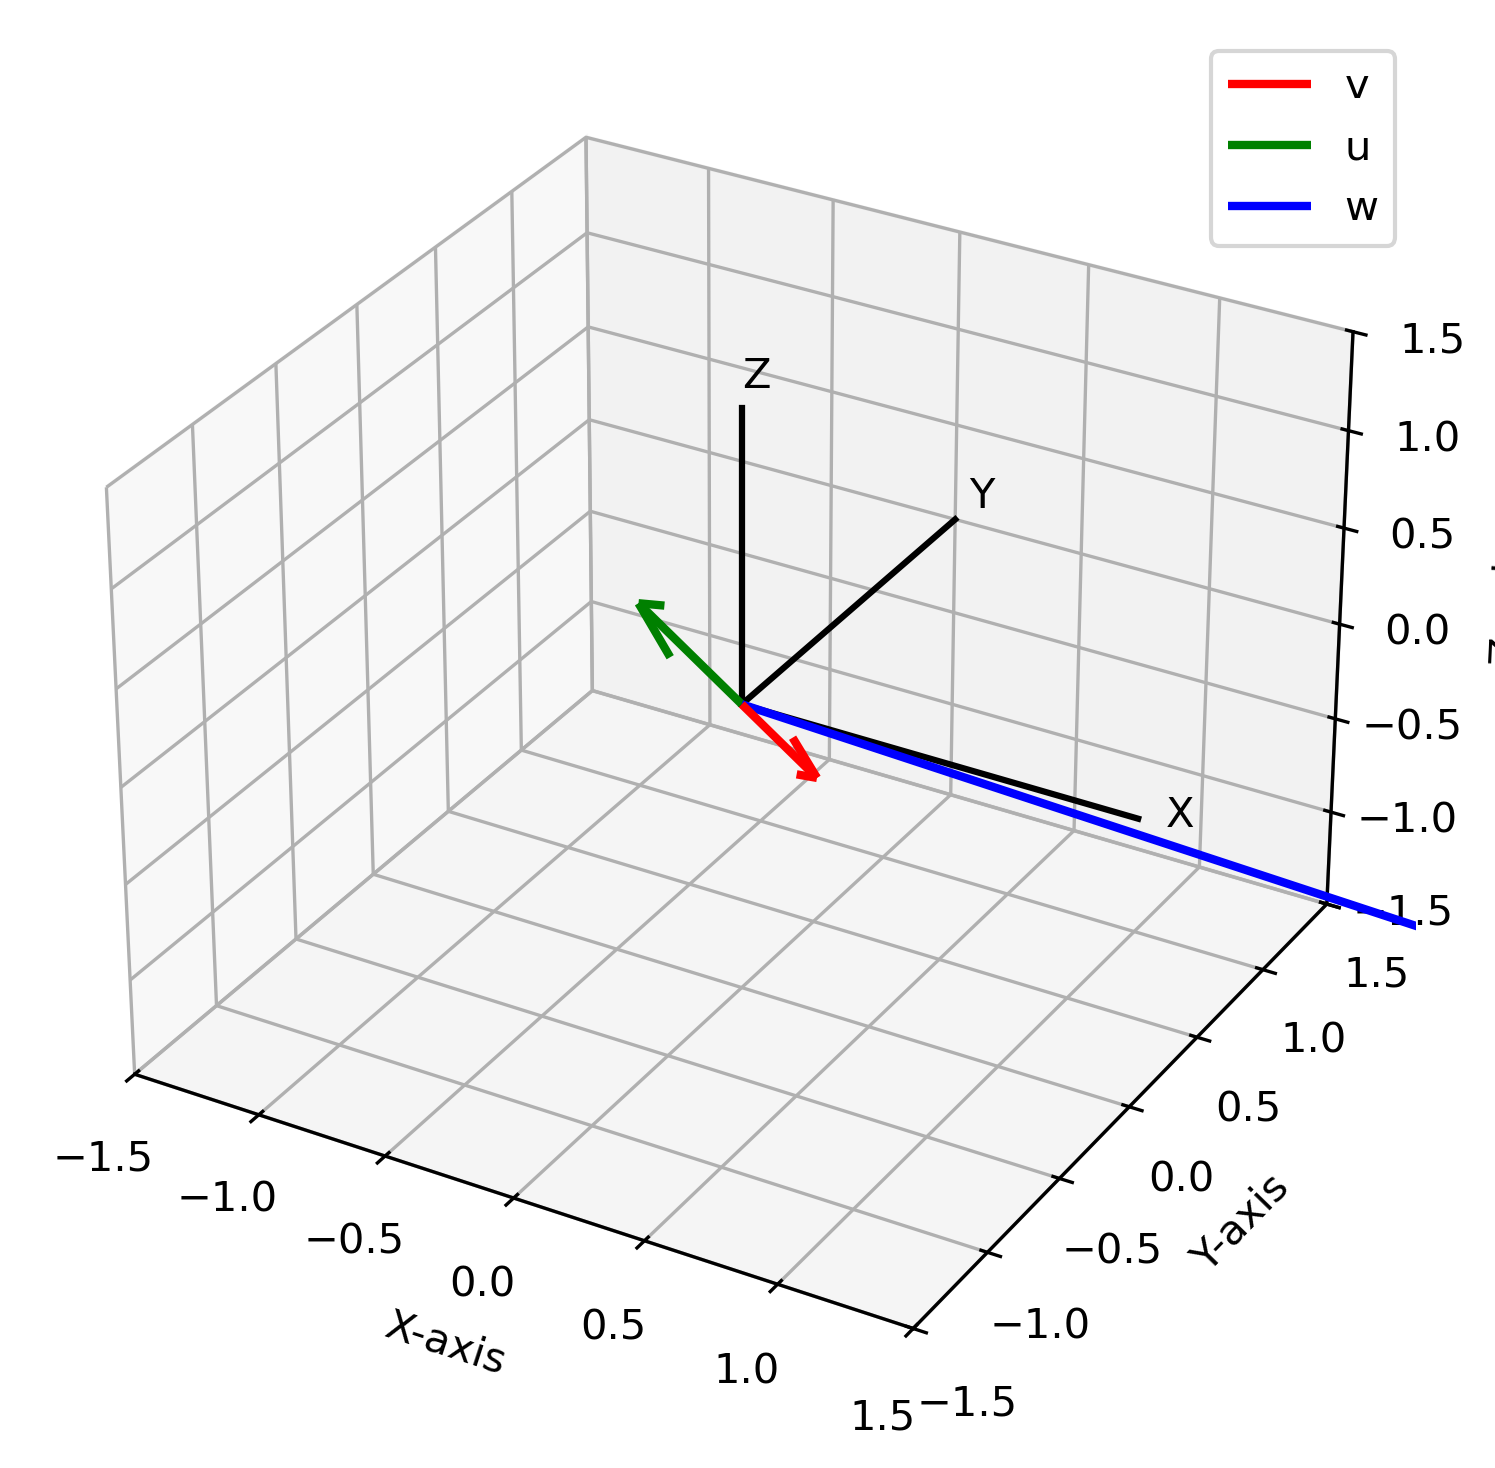
\includegraphics[width=\columnwidth, height=0.8\textheight, keepaspectratio]{figs/Figure_1.png}
\end{document}